\section{Evaluating GAN performance}
Evaluating the performance of a discriminative model is a rather straightforward issue. One would reserve a portion of the available data  for a test dataset and run the model on this dataset after the training finishes to count the number of correctly classified samples. With generative models things get more complicated. Measuring the quality of generated samples, whether these are images, text or something else, can be challenging and often subjective. Therefore, some creative ideas were proposed to tackle this problem. Some of the methods can be applied only in a particular domain, like generating images displaying multiple objects, while others can be applied to an arbitrary GAN. 
\subsection{Manual evaluation}
The best way to measure the quality of generated content is still by using real people. For example, Ian Goodfellow \textit{et al.} have created a simple website\footnote{The website can be accessed under  \url{http://infinite-chamber-35121.herokuapp.com/cifar-minibatch/}}, showing a user a number of pictures, some of which are generated and some are real. The user is then asked to choose the pictures which he or she thinks were generated by the network. Moreover, the quality of an image is also indicated by the time spent to decide whether it is real or not. Therefore, Emily Denton \textit{et al.} did several tests with different amounts of time user was able to look at an image before it disappeared~\cite{laplacian_gan}. If the number of positive responses declines with the increase of the amount of time available to examine an image, it is a signal of the poor image quality.

\subsection{Inception score}
The Inception score can be only applied to GANs used to generate objects from multiple categories. It uses the Inception network ~\cite{inception} to classify objects present on each image produced by a target GAN generator. Although any other network architecture could be used to do the classification, the Inception network has a relatively low number of parameters and therefore each classification takes less time, the exact precision of the network is not that important as long as it remains constant for all evaluations of the GAN performance. Using this classification we obtain a conditional label distribution for each generated image $p(y | x)$. The inception score is based on two characteristics we expect from a good generator:
\begin{enumerate}
	\item The Inception network should recognize few distinct objects in a generated image. This is equal to saying that entropy $H[p(y|x)]$ should be low.
	\item The generator should produce a large variety of images. Thus the entropy of marginal $p(y) = \int_z p(y|x=G(z))dz$ should be large. 
\end{enumerate}
Both these requirements can be verified by observing the value 
\begin{equation}
I(G) = \exp(\E_{x \sim p_g}[KL(p(y) \lVert p(y|x))]),
\end{equation}
where $KL$ denotes the Kullback-Leibler divergence and exponentiation is used to obtain a wider spectrum of values. 

\subsection{Generative adversarial metric(GAM)} \label{sec:gam}
Generative adversarial metric (GAM) is another way of comparing the performance of two GANs. This metric does not quantify the quality of a single GAN but rather can give a hint on which of two compared networks performs better. This is done by swapping the GAN discriminators, as shown in Figure~\ref{fig:gam}. 
\begin{figure}[h]
	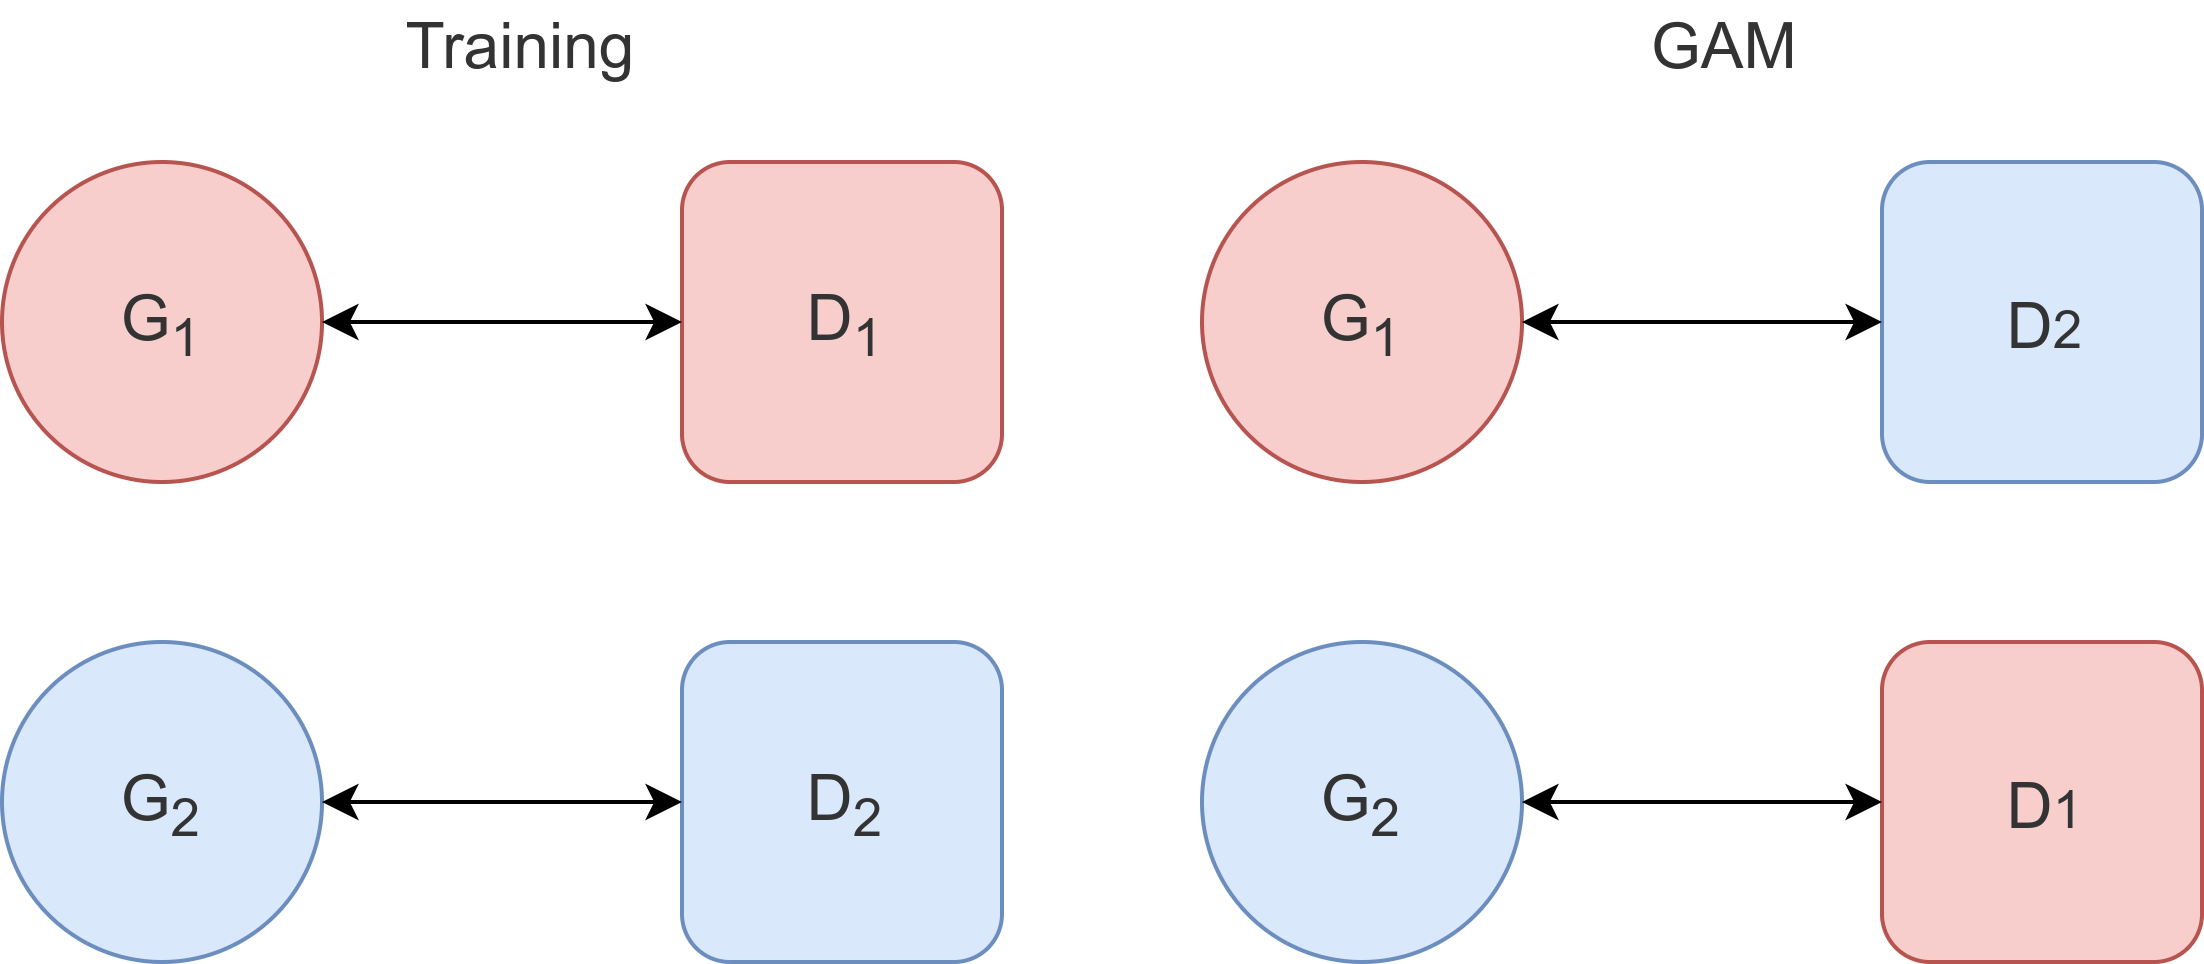
\includegraphics[width=\textwidth]{figures/gam}
	\caption{A visualization the GAM idea. The first GAN consists of a generator $G_1$ and a discriminator $D_1$, the second one of $G_2$ and $D_2$. When computing the GAM, GANs swap their discriminators, so that $D_1$ judges whether images data produced by $G_2$ look realistic or not, while $D_2$ does the same for $G_1$.}
	\label{fig:gam}
\end{figure}
 
After exchanging discriminators two quantities are computed:
\begin{align} \label{eq:gam_real}
	r_{real} &= \frac{\epsilon(D_1(x_{real}))}{\epsilon(D_2(x_{real}))} \\ 
	r_{generated} &= \frac{\epsilon(D_1(G_2(z)))}{\epsilon(D_2(G_1(z)))}, \label{eq:gam_gen} 
 \end{align}
where $\epsilon(\cdot)$ denotes the misclassification ratio which is be computed by 
\begin{equation*}
	\frac{\text{correctly classified samples}}{\text{total number of samples}}.
\end{equation*} 
Then, depending on the values of the two indicators, we can conclude which GAN performs better:
\begin{equation}
\text{winner} = \begin{cases}
	GAN_1, & \text{if } r_{generator} < 1 \text{ and } r_{real} \approx 1 \\
	GAN_2, & \text{if } r_{generator} > 1 \text{ and } r_{real} \approx 1 \\
	\text{tie}, & \text{if } r_{generator} \approx 1 \text{ and } r_{real} \approx 1  \\
	\text{undefined}, & \text{if } r_{real} \not \approx 1	
	\end{cases}
\end{equation}
Note that because we actually want to compare the generators, such a comparison is possible only if both discriminators perform equally well, which is indicated by the condition $r_{real} \approx 1$.  
